\documentclass[letterpaper,headings=standardclasses]{scrartcl}

\usepackage[margin=1in,includefoot]{geometry}
\usepackage{amssymb}
\usepackage{amsmath}
\usepackage{listings}
\usepackage{tikz}
\usepackage{float}
\usepackage[export]{adjustbox}

\usetikzlibrary{shapes,arrows}

\tikzset{
  block/.style    = {draw, thick, rectangle, minimum height = 3em, minimum width = 3em},
  sum/.style      = {draw, circle},
  input/.style    = {coordinate, circle},
  output/.style   = {coordinate, circle}
}

\lstset{basicstyle=\ttfamily,language=python,columns=flexible,breaklines=true}

\title{Homework 3}
\subtitle{CS 559 - Neural Networks - Fall 2019}
\author{Matteo Corain 650088272}

\begin{document}

\maketitle

\section{Question 1}

\subsection{Gradient and Hessian of $f$}

The gradient of the function $f(x,y) = -\log{(1-x-y)} -\log{x} - \log{y}$ may be computed as follows:

$$ \nabla f(x,y) = \left[ \begin{matrix} \frac{\partial f}{\partial x}(x,y) \\[0.5em] \frac{\partial f}{\partial y}(x,y) \end{matrix} \right] $$

$$ \frac{\partial f}{\partial x}(x,y) = -\frac{1}{1-x-y} \frac{\partial}{\partial x}(1-x-y) -\frac{1}{x} = \frac{1}{1-x-y} -\frac{1}{x} $$

$$ \frac{\partial f}{\partial y}(x,y) = -\frac{1}{1-x-y} \frac{\partial}{\partial y}(1-x-y) -\frac{1}{y} = \frac{1}{1-x-y} -\frac{1}{y} $$

$$ \nabla f(x,y) = \left[ \begin{matrix} \frac{1}{1-x-y} -\frac{1}{x} \\[0.5em] \frac{1}{1-x-y} -\frac{1}{y} \end{matrix} \right] $$

Starting from those result, the Hessian matrix of $f(x,y)$ may be computed as follows:

$$ Hf(x,y) = \left[ \begin{matrix} \frac{\partial^2 f}{\partial x^2}(x,y) & \frac{\partial^2 f}{\partial x \partial y}(x,y) \\[0.5em] \frac{\partial^2 f}{\partial y \partial x}(x,y) & \frac{\partial^2 f}{\partial y^2}(x,y) \end{matrix} \right] $$

$$ \frac{\partial^2 f}{\partial x^2}(x,y) = \frac{\partial}{\partial x} \frac{\partial f}{\partial x} = - \frac{1}{(1-x-y)^2} \frac{\partial}{\partial x}(1-x-y) + \frac{1}{x^2} = \frac{1}{(1-x-y)^2} + \frac{1}{x^2} $$

$$ \frac{\partial^2 f}{\partial x \partial y}(x,y) = \frac{\partial}{\partial x} \frac{\partial f}{\partial y} = - \frac{1}{(1-x-y)^2} \frac{\partial}{\partial x}(1-x-y) = \frac{1}{(1-x-y)^2} $$

$$ \frac{\partial^2 f}{\partial y \partial x}(x,y) = \frac{\partial}{\partial y} \frac{\partial f}{\partial x} = - \frac{1}{(1-x-y)^2} \frac{\partial}{\partial y}(1-x-y) = \frac{1}{(1-x-y)^2} $$

$$ \frac{\partial^2 f}{\partial y^2}(x,y) = \frac{\partial}{\partial y} \frac{\partial f}{\partial y} = - \frac{1}{(1-x-y)^2} \frac{\partial}{\partial y}(1-x-y) + \frac{1}{y^2} = \frac{1}{(1-x-y)^2} + \frac{1}{y^2} $$

$$ Hf(x,y) = \left[ \begin{matrix} \frac{1}{(1-x-y)^2} + \frac{1}{x^2} & \frac{1}{(1-x-y)^2} \\[0.5em] \frac{1}{(1-x-y)^2} & \frac{1}{(1-x-y)^2} + \frac{1}{y^2} \end{matrix} \right] $$

Using the obtained results, it is possible to analytically compute where the minimum of the given function is located; in fact, this correspond to the point $(x,y)$ for which we have $\nabla f(x,y) = 0$. This condition is equivalent to the solution of the following system of equalities:

$$ \nabla f(x,y) = 0 \Rightarrow \begin{cases} \frac{\partial f}{\partial x}(x,y) = \frac{1}{1-x-y} -\frac{1}{x} = 0 \\ \frac{\partial f}{\partial y}(x,y) = \frac{1}{1-x-y} -\frac{1}{y} = 0 \end{cases} \Rightarrow \left[ \begin{matrix} x \\ y \end{matrix} \right] = \left[ \begin{matrix} \frac{1}{3} \\[0.5em] \frac{1}{3} \end{matrix} \right] $$

We expect therefore that both the gradient descent and the Newton's methods will be able to converge to points in the neighborhood of $\left( \frac{1}{3}, \frac{1}{3} \right)$.

\subsection{Gradient descent method}

The gradient descent method is based on the update rule:

$$ \left[ \begin{matrix} x_{n+1} \\ y_{n+1} \end{matrix} \right] \leftarrow \left[ \begin{matrix} x_n \\ y_n \end{matrix} \right] - \eta \nabla f(x_n, y_n) $$

This method was implemented in code using the \texttt{gdesc()} function, which takes as arguments the initial point $(x_0, y_0)$, the value of $\eta$ and the value of $\epsilon$, which defines the minimum entity of the update before stopping the iterations.

At each iteration, the function updates the estimate of the minimum, appends to the array \texttt{xylist} the value of the updated point and to the array \texttt{fxy} the value of the function in correspondence of that updated point. At convergence, the algorithm returns the final estimate and the two lists \texttt{xylist} and \texttt{fxy}.

Results are then plotted using the \texttt{plot\_traj()} and \texttt{plot\_fxy()} functions. The first creates a new 3D figure, defines a triangular grid inside the domain $\mathcal{D}$ of the function (keeping distance $\delta$ from the domain boundaries and with the given step) and plots both the function and the sequence of weights onto that plot. The global minimum is also drawn on the obtained graph. The second function performs a simple 2D plot operation of the given vector.

Obtained results are shown in figures \ref{gd_graph} and \ref{gd_fval}. Those were computed starting from the initial point $ (x_0, y_0) = [\begin{matrix} 0.90348 & 0.03794 \end{matrix}] $, decreasing the value of $\eta$ to 0.01 in order not to make the point jump outside $\mathcal{D}$ and using $\epsilon = 10^{-6}$.

\subsection{Newton's method}

The Newton's method is based on the weights update rule:

$$ \left[ \begin{matrix} x_{n+1} \\ y_{n+1} \end{matrix} \right] \leftarrow \left[ \begin{matrix} x_n \\ y_n \end{matrix} \right] - \eta [Hf(x_n, y_n)]^{-1} \nabla f(x_n,y_n) $$

This method was implemented in code using the \texttt{newton()} function, which performs similar action with respect to the one implementing gradient descent. The same functions are used for plotting. The method was made run using the same initial point $(x_0, y_0)$ and minimum update $\epsilon$ as before, but using learning parameter $\eta = 1$; results are shown in figures \ref{nm_graph} and \ref{nm_fval}.

\pagebreak

\begin{figure}[H]
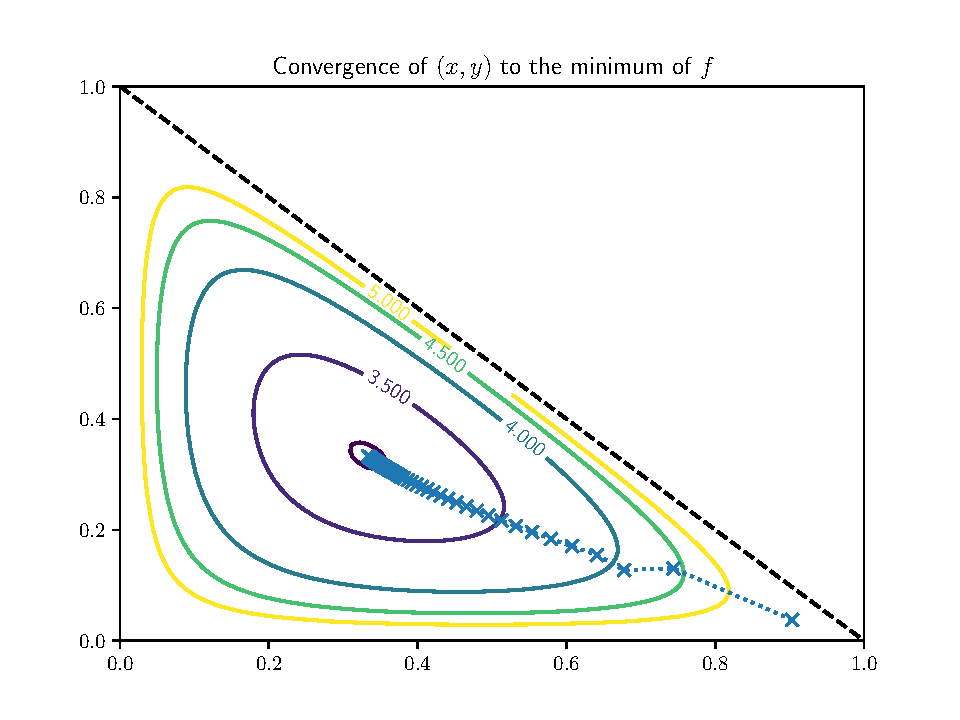
\includegraphics[width=1.2\linewidth,center]{gd_graph.pdf}
\caption{Convergence using gradient descent method}
\label{gd_graph}
\end{figure}

\begin{figure}[H]
\centering
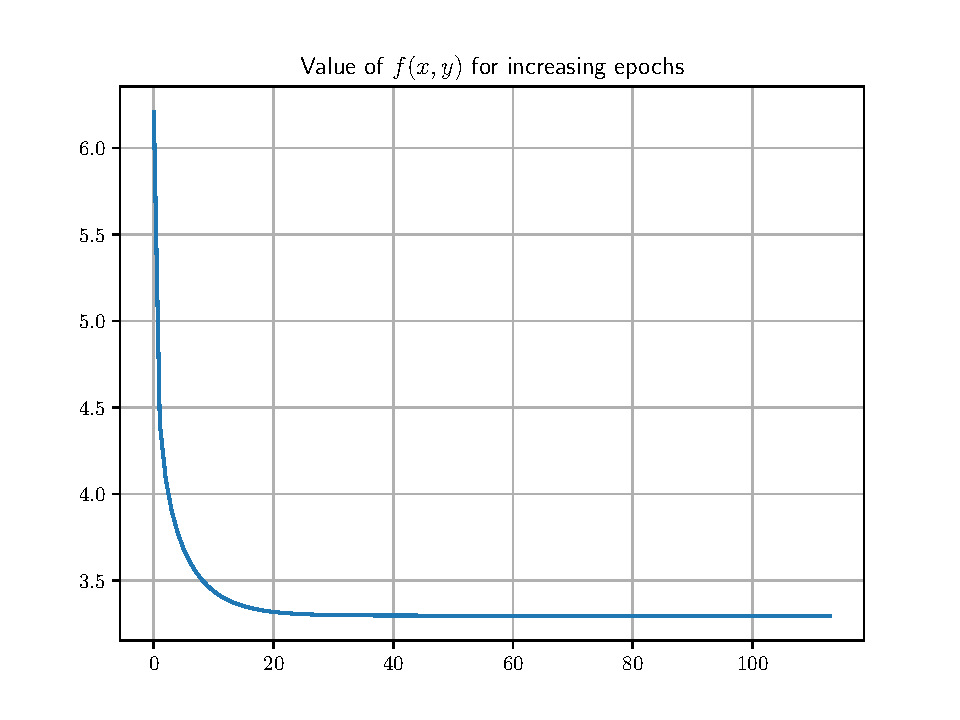
\includegraphics[width=.6\linewidth]{gd_fval.pdf}
\caption{Decrease of $f$-values using gradient descent method}
\label{gd_fval}
\end{figure}

\begin{figure}[H]
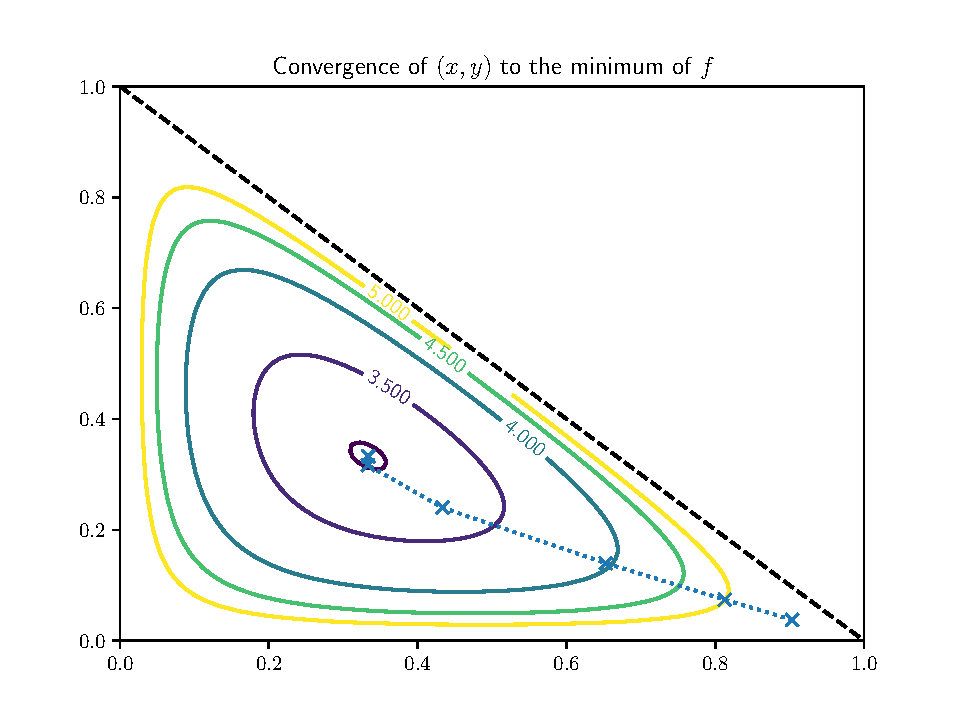
\includegraphics[width=1.2\linewidth,center]{nm_graph.pdf}
\caption{Convergence using Newton's method}
\label{nm_graph}
\end{figure}

\begin{figure}[H]
\centering
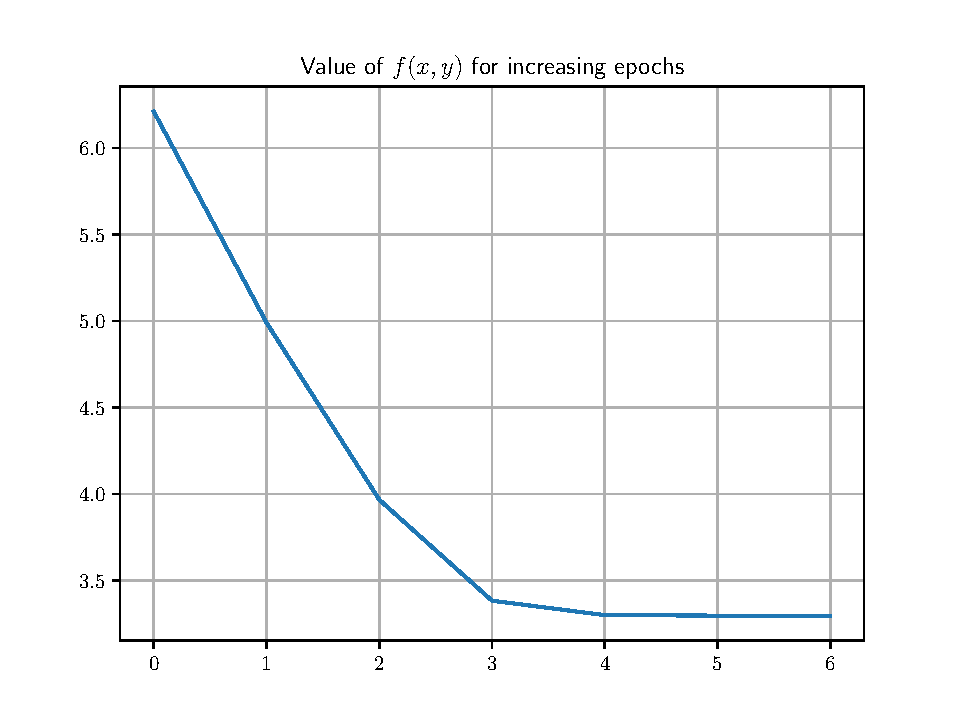
\includegraphics[width=.6\linewidth]{nm_fval.pdf}
\caption{Decrease of $f$-values using Newton's method}
\label{nm_fval}
\end{figure}

\subsection{Comparison}

\begin{table}[h]
\centering
\begin{tabular}{|c|c|c|c|}
\hline
Method           & $\eta$ & Epochs & Convergence value \\ \hline
Gradient descent & 0.01   & 114    & $[\begin{matrix} 0.33334089 & 0.33332578 \end{matrix}]$ \\ \hline
Newton           & 1      & 7      & $[\begin{matrix} 0.33333286 & 0.33333348 \end{matrix}]$ \\ \hline
\end{tabular}
\caption{Summary of the results obtained using gradient descent and Newton's method}
\label{summ_res}
\end{table}

As it can be seen from the summary of the results, Newton's method was able to converge in a much lower number of epochs and with a much higher precision to the minimum of $f(x,y)$.

\subsection{Complete Python code}

\lstinputlisting[basicstyle=\ttfamily\scriptsize]{hw3_ex1.py}

\section{Question 2}

\subsection{Linear least squares fit}

The values for the parameters $w_0$ and $w_1$ of the linear least squares fit for the given data set can be obtained by minimizing the value of:

$$ E = \sum_{i = 1}^{50} (y_i - (w_0 + w_1 x_i))^2 $$

Let us rewrite this expression by introducing the matrices:

$$ X = \left[ \begin{matrix} 1 & 1 & \dots & 1 \\ x_1 & x_2 & \dots & x_{50} \end{matrix} \right], Y = \left[ \begin{matrix} y_1 & y_2 & \dots & y_{50} \end{matrix} \right] $$

$$ \Rightarrow E = \sum_{i = 1}^{50} (y_i - (w_0 + w_1 x_i))^2 = || Y - WX ||^2 $$

This corresponds to a simple linear optimization problem, which can be solved in a closed form using the pseudoinverse method:

$$ W = YX^{+} $$

Where $X^{+}$ denotes the Moore-Penrose pseudoinverse of $X$. Given that this $X$ has linearly independent rows, the pseudoinverse $X^{+}$ may be computed as:

\begin{multline*}
X^{+} = X^T \left( XX^T \right)^{-1} = \left[ \begin{matrix} 1 & x_1 \\ 1 & x_2 \\ \vdots & \vdots \\ 1 & x_{50} \end{matrix} \right] \left( \left[ \begin{matrix} 1 & 1 & \dots & 1 \\ x_1 & x_2 & \dots & x_{50} \end{matrix} \right] \left[ \begin{matrix} 1 & x_1 \\ 1 & x_2 \\ \vdots & \vdots \\ 1 & x_{50} \end{matrix} \right] \right)^{-1} \\
= \left[ \begin{matrix} 1 & x_1 \\ 1 & x_2 \\ \vdots & \vdots \\ 1 & x_{50} \end{matrix} \right] \left[ \begin{matrix} 50 & \sum_{i = 1}^{50} x_i \\[0.5em] \sum_{i = 1}^{50} x_i & \sum_{i = 1}^{50} x_i^2 \end{matrix} \right]^{-1} = \frac{1}{50 \sum_{i = 1}^{50} x_i^2 - \left( \sum_{i = 1}^{50} x_i \right)^2} \left[ \begin{matrix} 1 & x_1 \\ 1 & x_2 \\ \vdots & \vdots \\ 1 & x_{50} \end{matrix} \right] \left[ \begin{matrix} \sum_{i = 1}^{50} x_i^2 & -\sum_{i = 1}^{50} x_i \\[0.5em] -\sum_{i = 1}^{50} x_i & 50 \end{matrix} \right] \\
= \frac{1}{50 \sum_{i = 1}^{50} x_i^2 - \left( \sum_{i = 1}^{50} x_i \right)^2} \left[ \begin{matrix} \sum_{i = 1}^{50} x_i^2 - x_1 \sum_{i = 1}^{50} x_i & -\sum_{i = 1}^{50} x_i + 50 x_1 \\[0.5em] \sum_{i = 1}^{50} x_i^2 - x_2 \sum_{i = 1}^{50} x_i & -\sum_{i = 1}^{50} x_i + 50 x_2 \\[0.5em] \vdots & \vdots \\[0.5em] \sum_{i = 1}^{50} x_i^2 - x_{50} \sum_{i = 1}^{50} x_i & -\sum_{i = 1}^{50} x_i + 50 x_{50} \end{matrix} \right]
\end{multline*}

Therefore, the analytic solution of this optimization problem is:

\begin{multline*}
W = YX^{+} = \frac{\left[ \begin{matrix} y_1 & y_2 & \dots & y_{50} \end{matrix} \right]}{50 \sum_{i = 1}^{50} x_i^2 - \left( \sum_{i = 1}^{50} x_i \right)^2} \left[ \begin{matrix} \sum_{i = 1}^{50} x_i^2 - x_1 \sum_{i = 1}^{50} x_i & -\sum_{i = 1}^{50} x_i + 50 x_1 \\[0.5em] \sum_{i = 1}^{50} x_i^2 - x_2 \sum_{i = 1}^{50} x_i & -\sum_{i = 1}^{50} x_i + 50 x_2 \\[0.5em] \vdots & \vdots \\[0.5em] \sum_{i = 1}^{50} x_i^2 - x_{50} \sum_{i = 1}^{50} x_i & -\sum_{i = 1}^{50} x_i + 50 x_{50} \end{matrix} \right] \\
= \left[ \begin{matrix} \frac{\textstyle \sum_{i = 1}^{50} x_i^2 \sum_{i = 1}^{50} y_i - \sum_{i = 1}^{50} x_i \sum_{i = 1}^{50} x_i y_i}{\textstyle 50 \sum_{i = 1}^{50} x_i - \left( \sum_{i = 1}^{50} x_i \right)^2} & \frac{\textstyle -\sum_{i = 1}^{50} x_i^2 \sum_{i = 1}^{50} y_i + 50 \sum_{i = 1}^{50} x_i y_i}{\textstyle 50 \sum_{i = 1}^{50} x_i - \left( \sum_{i = 1}^{50} x_i \right)^2} \end{matrix} \right]
\end{multline*}

Applying the presented formulas on a randomly generated dataset (the random seed is fixed for reproducibility), we obtain the following values for the linear interpolation coefficients:

$$ w_0 = 0.15612 $$
$$ w_1 = 0.99762 $$

Figure \ref{lls} shows the approximation line computed using the least squares method.

\begin{figure}[h]
\centering
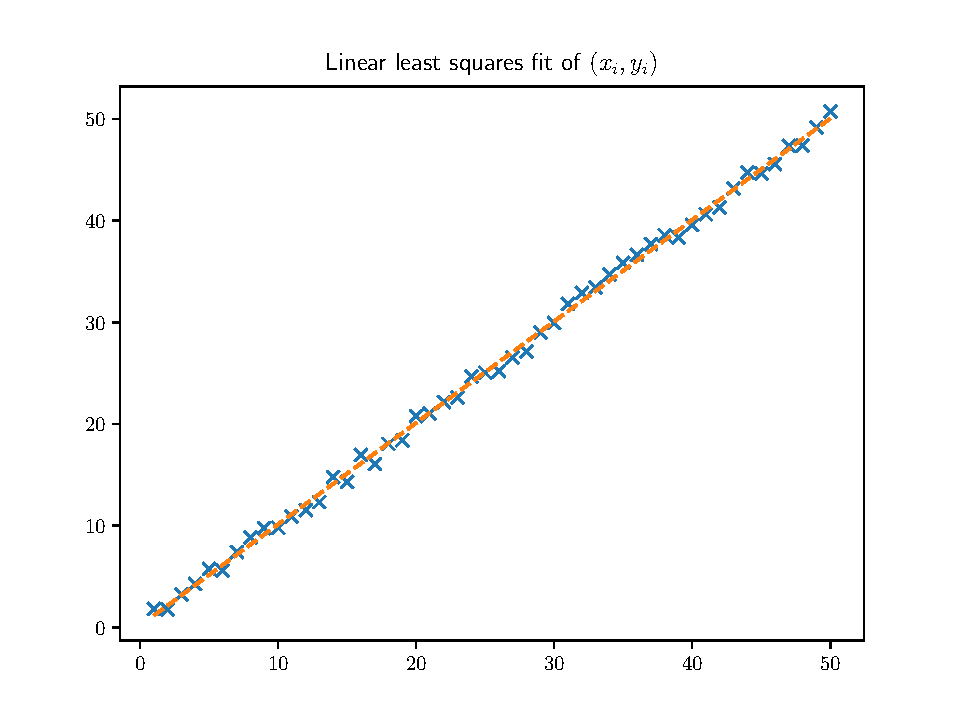
\includegraphics[width=.7\linewidth]{lls.pdf}
\caption{Linear least squares fit of points $(x_i, y_i)$}
\label{lls}
\end{figure}

\subsection{Gradient descent method}

Let us recall that the gradient descent method is based on the weights update rule:

$$ w \leftarrow w - \eta \nabla E $$

In our case, as obtained before:

$$ \nabla E = \left[ \begin{matrix} -2 \sum_{i = 1}^{50} (y_i - (w_0 + w_1 x_i)) & -2 \sum_{i = 1}^{50} x_i (y_i - (w_0 + w_1 x_i)) \end{matrix} \right]^T $$

Using as the stopping condition of the algorithm a minimum norm for the update term set to $\epsilon = 10^{-6}$, the gradient descent method converges (using $\eta = 2.25 * 10^{-5}$) to the following weights:

$$ w_0 = 0.15429 $$
$$ w_1 = 0.99767 $$

Those values are actually quite similar to the ones computed when solving the equations in a closed form, and they can possibly be even closer if we decreased furtherly the value of $\epsilon$. In fact, we expect that it would be possible to approximate the regression coefficients as computed using the method of the linear least squares fit with arbitrary precision, if we can afford to make the algorithm run for a sufficient number of epochs.

\subsection{Newton's method}

Let us recall that the Newton's method is based on the weights update rule:

$$ w \leftarrow w - \eta [HE]^{-1} \nabla E $$

The Hessian matrix of $E$ can be computed as follows:

$$ HE = \left[ \begin{matrix} \frac{\partial^2 E}{\partial w_0^2} & \frac{\partial^2 E}{\partial w_0 \partial w_1} \\[0.5em] \frac{\partial^2 E}{\partial w_1 \partial w_0} & \frac{\partial^2 E}{\partial w_1^2} \end{matrix} \right] = \left[ \begin{matrix} \frac{\partial}{\partial w_0} \frac{\partial E}{\partial w_0} & \frac{\partial}{\partial w_0} \frac{\partial E}{\partial w_1} \\[0.5em] \frac{\partial}{\partial w_1} \frac{\partial E}{\partial w_0} & \frac{\partial}{\partial w_1} \frac{\partial E}{\partial w_1} \end{matrix} \right] = \left[ \begin{matrix} 100 & 2 \sum_{i = 1}^{50} x_i \\[0.5em] 2 \sum_{i = 1}^{50} x_i & 2 \sum_{i = 1}^{50} x_i^2 \end{matrix} \right] $$

It can be verified that, after a single epoch using $\eta = 1$, this method makes the weights $w$ converge to the global minimum of $E$:

$$ w_0 = 0.15612 $$
$$ w_1 = 0.99762 $$

This result was expected since function $E$ is quadratic: this means that its local quadratic approximation corresponds, in any point, to the function itself. Therefore, since each iteration of the Newton's method moves the weights to the minimum of the function's quadratic approximation around $w$, a single iteration is needed to converge to the global minimum of $E$, independently on the initial selection of weights.

It is also possible to derive those results analytically by writing the expression of the weights after the update; in the following, $w_0$ and $w_1$ denote the initial weights (before the update), while $w_0'$ and $w_1'$ denote the weights after a single update using Newton's method:

\begin{multline*}
\left[ \begin{matrix} w_0' \\ w_1' \end{matrix} \right] = w - \eta [HE]^{-1} \nabla E = \\
\left[ \begin{matrix} w_0 \\ w_1 \end{matrix} \right] - \frac{1}{200 \sum_{i = 1}^{50} x_i^2 - 4 \left[ \sum_{i = 1}^{50} x_i \right]^2} \left[ \begin{matrix} 2 \sum_{i = 1}^{50} x_i^2 & -2 \sum_{i = 1}^{50} x_i \\[0.5em] -2 \sum_{i = 1}^{50} x_i & 100 \end{matrix} \right] \left[ \begin{matrix} -2 \sum_{i = 1}^{50} (y_i - (w_0 + w_1 x_i)) \\ -2 \sum_{i = 1}^{50} x_i (y_i - (w_0 + w_1 x_i)) \end{matrix} \right]
\end{multline*}

\begin{multline*}
w_0' = w_0 - \frac{-4 \sum_{i = 1}^{50} x_i^2 \sum_{i = 1}^{50} (y_i - w_0 - w_1 x_i) + 4 \sum_{i = 1}^{50} x_i \sum_{i = 1}^{50} x_i(y_i - w_0 - w_1 x_i)}{200 \sum_{i = 1}^{50} x_i^2 - 4 \left[ \sum_{i = 1}^{50} x_i \right]^2} \\
%= \frac{200 w_0 \sum_{i = 1}^{50} x_i^2 - 4 w_0 \left[ \sum_{i = 1}^{50} x_i \right]^2 + 4 \sum_{i = 1}^{50} x_i^2 \sum_{i = 1}^{50} y_i - 200 \sum_{i = 1}{50} x_i^2 - 4 w_1 \sum_{i = 1}^{50} x_i^2 \sum_{i = 1}^{50} x_i - 4 \sum_{i = 1}^{50} x_i \sum_{i = 1}^{50} x_i y_i + 4 w_0 \left[ \sum_{i = 1}^{50} x_i \right]^2 + 4 w_1 \sum_{i = 1}^{50} x_i \sum_{i = 1}^{50} x_i^2}{200 \sum_{i = 1}^{50} x_i^2 - 4 \left[ \sum_{i = 1}^{50} x_i \right]^2} \\
= \frac{4 \sum_{i = 1}^{50} x_i^2 \sum_{i = 1}^{50} y_i - 4 \sum_{i = 1}^{50} x_i \sum_{i = 1}^{50} x_i y_i}{200 \sum_{i = 1}^{50} x_i^2 - 4 \left[ \sum_{i = 1}^{50} x_i \right]^2} = \frac{\sum_{i = 1}^{50} x_i^2 \sum_{i = 1}^{50} y_i - \sum_{i = 1}^{50} x_i \sum_{i = 1}^{50} x_i y_i}{50 \sum_{i = 1}^{50} x_i^2 - \left[ \sum_{i = 1}^{50} x_i \right]^2}
\end{multline*}

\begin{multline*}
w_1' = w_1 - \frac{4 \sum_{i = 1}^{50} x_i \sum_{i = 1}^{50} (y_i - w_0 - w_1 x_i) - 200 \sum_{i = 1}^{50} x_i(y_i - w_0 - w_1 x_i)}{200 \sum_{i = 1}^{50} x_i^2 - 4 \left[ \sum_{i = 1}^{50} x_i \right]^2} \\
%= \frac{200 w_1 \sum_{i = 1}^{50} x_i^2 - 4 w_1 \left[ \sum_{i = 1}^{50} x_i \right]^2 - 4 \sum_{i = 1}^{50} x_i \sum_{i = 1}^{50} y_i + 200 w_0 \sum_{i = 1}^{50} x_i + 4 w_1 \left[ \sum_{i = 1}^{50} x_i \right]^2 + 200 \sum_{i = 1}^{50} x_i y_i - 200 w_0 \sum_{i = 1}^{50} x_i - 200 w_1 \sum_{i = 1}^{50} x_i^2}{200 \sum_{i = 1}^{50} x_i^2 - 4 \left[ \sum_{i = 1}^{50} x_i \right]^2} \\
= \frac{-4 \sum_{i = 1}^{50} x_i \sum_{i = 1}^{50} y_i + 200 \sum_{i = 1}^{50} x_i y_i}{200 \sum_{i = 1}^{50} x_i^2 - 4 \left[ \sum_{i = 1}^{50} x_i \right]^2} = \frac{50 \sum_{i = 1}^{50} x_i y_i - \sum_{i = 1}^{50} x_i \sum_{i = 1}^{50} y_i}{50 \sum_{i = 1}^{50} x_i^2 - \left[ \sum_{i = 1}^{50} x_i \right]^2}
\end{multline*}

As it can be seen, the expression of the weights after a single update using Newton's method does not depend on the initial value of $w_0$ and $w_1$ and, most importantly, is analogous to the one derived for solving the linear least squares problem.

\subsection{Complete Python code}

\lstinputlisting[basicstyle=\ttfamily\scriptsize]{hw3_ex2.py}

\end{document}